\documentclass[11pt]{article}

% use packages
\usepackage[utf8]{inputenc}
\usepackage{amsmath}
\usepackage{amsthm}
\usepackage{amsfonts}
\usepackage{amscd}
\usepackage{amssymb}
\usepackage{natbib}
\usepackage{url}

\usepackage{graphicx}
%\usepackage{mathtools}
\usepackage{enumitem}
\usepackage{authblk}
\usepackage{bm}
\usepackage[usenames]{color}
\usepackage{hyperref}

\usepackage{caption}
\usepackage{float}
\usepackage[caption = false]{subfig}
\usepackage{tikz}
\usepackage{multirow}
\usepackage[linesnumbered, ruled,vlined]{algorithm2e}
\usepackage{pdflscape}

% margin setup
\usepackage{geometry}
\geometry{margin=0.8in}


% function definition
\newcommand{\R}{\mathbb{R}}
\newcommand{\w}{\textbf{w}}
\newcommand{\x}{\textbf{x}}
\newcommand{\dbf}{\textbf{d}}
\newcommand{\y}{\textbf{y}}
\newcommand{\X}{\textbf{X}}
\newcommand{\Y}{\textbf{Y}}
\newcommand{\L}{\textbf{L}}
\newcommand{\Hist}{\mathcal{H}}
\newcommand{\Prob}{\mathbb{P}}
\def\mbf#1{\mathbf{#1}} % bold but not italic
\def\ind#1{\mathrm{1}(#1)} % indicator function
\newcommand{\simiid}{\stackrel{iid}{\sim}} %[] IID 
\def\where{\text{ where }} % where
\newcommand{\indep}{\perp \!\!\! \perp } % independent symbols
\def\cov#1#2{\mathrm{Cov}(#1, #2)} % covariance 
\def\mrm#1{\mathrm{#1}} % remove math
\newcommand{\reals}{\mathbb{R}} % Real number symbol
\def\t#1{\tilde{#1}} % tilde
\def\normal#1#2{\mathcal{N}(#1,#2)} % normal
\def\mbi#1{\boldsymbol{#1}} % Bold and italic (math bold italic)
\def\v#1{\mbi{#1}} % Vector notation
\def\mc#1{\mathcal{#1}} % mathical
\DeclareMathOperator*{\argmax}{arg\,max} % arg max
\DeclareMathOperator*{\argmin}{arg\,min} % arg min
\def\E{\mathbb{E}} % Expectation symbol
\def\mc#1{\mathcal{#1}}
\def\var#1{\mathrm{Var}(#1)} % Variance symbol
\def\checkmark{\tikz\fill[scale=0.4](0,.35) -- (.25,0) -- (1,.7) -- (.25,.15) -- cycle;} % checkmark
\newcommand\red[1]{{\color{red}#1}}
\def\bs#1{\boldsymbol{#1}}
\def\P{\mathbb{P}}
\def\var{\mathbf{Var}}
\def\naturals{\mathbb{N}}
\def\cp{\overset{p}{\to}}
\def\clt{\overset{\mathcal{L}^2}{\to}}

\setcounter{tocdepth}{4}
\setcounter{secnumdepth}{4}

\newtheorem{corollary}{Corollary}
\newcommand{\ceil}[1]{\lceil #1 \rceil}
\newcommand{\norm}[1]{\left\lVert#1\right\rVert} % A norm with 1 argument
\DeclareMathOperator{\Var}{Var} % Variance symbol

\newtheorem{cor}{Corollary}
\newtheorem{lem}{Lemma}
\newtheorem{thm}{Theorem}
\newtheorem{defn}{Definition}
\newtheorem{prop}{Proposition}
\theoremstyle{definition}
\newtheorem{remark}{Remark}
\hypersetup{
  linkcolor  = blue,
  citecolor  = blue,
  urlcolor   = blue,
  colorlinks = true,
} % color setup

% proof to proposition 
\newenvironment{proof-of-proposition}[1][{}]{\noindent{\bf
    Proof of Proposition {#1}}
  \hspace*{.5em}}{\qed\bigskip\\}
% general proof of corollary
  \newenvironment{proof-of-corollary}[1][{}]{\noindent{\bf
    Proof of Corollary {#1}}
  \hspace*{.5em}}{\qed\bigskip\\}
% general proof of lemma
  \newenvironment{proof-of-lemma}[1][{}]{\noindent{\bf
    Proof of Lemma {#1}}
  \hspace*{.5em}}{\qed\bigskip\\}

\allowdisplaybreaks

\title{Post-shock Volatility Forecasting Using Aggregated Shock Information}
\author{David Lundquist\thanks{davidl11@ilinois.edu} }
\affil{Department of Statistics, University of Illinois at Urbana-Champaign}
\date{December 3rd, 2021}

\begin{document}

\maketitle

\begin{abstract}
We develop a novel procedure for forecasting the volatility of a time series under study immediately following an exogenous shock event.  Adapting the synthetic prediction framework of \citet{lin2021minimizing}, we exploit series that have experienced similar shock events.  We extract volatility signals from these series in order to aggregate properly their shock-induced excess volatilities.  The volatility spikes are modeled as random effects and estimated as fixed effects.  The aggregation of these estimates is in service of adjusting the 1-step-ahead GARCH forecast of the time series under study by an additive term.  The adjusted and unadjusted forecasts are evaluated using three families of benchmarks: the unobservable but easily estimated realized volatility (RV) of the time series under study, implied volatility, and the empirical volatility over horizons of varying length.  We also compare the performance of the adjusted forecast to the performance of the Realized GARCH forecast, which is known to react faster to rapidly changing volatility than the standard GARCH model by permitting the inclusion of metrics like implied volatility.   Finally, we combine Realized GARCH modeling with the synthetic prediction framework, using Realized GARCH in both the estimation of random effects as well as the forecast for the time series under study.  Real world illustrations are provided, as are simulation results suggesting the conditions under which our approach's hyperparameters can be tuned for best performance.
\end{abstract}


\section{Introduction}

The most important stochastic phenomenon of many time series $(P_{t})_{t\in\mathbb{N}}$, especially financial time series, is the volatility of the return series of $(P_{t})_{t\in\mathbb{N}}$.  A financial asset's price series and daily return series may exhibit behavior that makes inconvenient and uninterpretable the traditional methods of time series analysis.  In contrast, the volatility of the return series may be less noisy, less structurally dependent on external factors, and more easily modeled as a weakly stationary process.  Yet even if one could model and forecast price series and return series with high accuracy, that would not necessarily tell us much about the variability of such forecasts nor enlighten us about the evolution of the variability of $(P_{t})_{t\in\mathbb{N}}$ over time. Modern portfolio management and theory requires information about at least the first two moments of a return series, if not higher.  For these reasons and others, volatility modeling has come to dominate financial econometrics over the past four decades.  

When $(P_{t})_{t\in\mathbb{N}}$ is positive, as one would expect of a price series, the percentage change over any interval of length $k\in\mathbb{N}$ can be approximated by $\text{log}(\frac{P_{t+k}}{P_{t}})$, owing to the fact that for any nonnegative real number y, $\text{log}(y+1)\leq y$.  Equality holds at exactly y = 0, corresponding to the case where $P_{t+k} = P_{t}$.  It is easily verified that the approximation works well when the ratio $\frac{P_{t+k}}{P_{t}} \in (.85,1.15)$, a return absolute value of $15\%$ or less.  The daily log return series $\text{log}(\frac{P_{t+1}}{P_{t}})$, however, not only provides an approximation to the daily return; the logarithm of a price series has the helpful property of being supported on $\mathbb{R}$.  Partly due to that, it earns a pedigree for its role in geometric Brownian motion, the foundation of much of modern financial mathematics, including the Black-Sholes differential equation \citep{tsay2005analysis}.  Additionally, the log transformation is a tried-and-true variance-reduction technique for heteroskedastic data \citep{faraway2016extending} and non-stationary time series.  In many applications, the log-return of a positive time series will allow us to reject the null of a unit-root process using the methods pioneered in \citet{dickey1979distribution} and \citet{dickey1981likelihood}, thus paving the way for the vast family of autoregressive-moving-average models.

However, no matter how a time series or its transformations is modeled, forecasting in the prescence of exogenous shock events requires a methodological framework that sensibly incorporates relevant information that has yet to manifest itself in market price or derivative quantities like volatility.  In this setting, regime-change models are of little use because under the assumption of a known exogenous shock, there is no need to estimate a regime-change time, nor is there data following the exogenous shock event to fit a model.  Asymmetric GARCH models were an early attempt to account for fact that negative returns typically beget larger volatility than positive returns \citep{hansen2012realized}.  As a separate problem, GARCH models have been shown slow to adapt to spikes in volatility (find first authors to point this out).  \citet{engle2002new} explored the use of implied volatility as an external regressor in a GARCH model, that is, using so-called GARCH-X models. \citet{hansen2012realized} propose Realized Garch, which aims to solve both the asymmetry problem as well as the slow-reaction problem by introducing a "measurement equation" as a tool for modeling the contribution to the conditional variance made by the market-implied volatility measure.  The key insight is that that the market-implied volatility measure is not independent of the conditional variance posited by the GARCH model.  Therefore, including the external measure must be done in a way that accounts for this dependence.

The approach herein can be viewed as an attempt to sidestep the functional complexity posited by Realized GARCH by substituting modeling assumptions.  Synthetic volatility forecasting proceeds under the assumption that similar exogenous shock events occasion volatility shocks arising from a common shock distribution.


\section{Setting}

\label{section2}

We follow convention and define the daily log-return as $r_{t} = \text{log}(\frac{P_{t+1}}{P_{t}})$.  The class of ARIMA(p,d,q) models developed in the mid-to-late 20th century provides a framework for postulating and quantifying the autoregressive structure of a $r_{t}$, all within the framework of frequentist statistics and maximum-likelihood estimation of parameters.  These models assume a certain dependence structure between $r_{t}$ and $r_{t-\text{max\{p,q\}}}$, as well as all observations in between, yet their errors -- often called innovations in the financial time series context due to how they represent the impact of new information -- are nevertheless assumed to be i.i.d. with mean zero and constant variance.  The ARCH \citep{engle1982autoregressive} and GARCH \citep{bollerslev1986generalized} models provide elegant alternatives to the constant-variance assumption.  In fact, the GARCH framework in its most basic form disregards $r_{t}$ and instead turns its interest to the series $r_{t}^{2}$ (when properly centered, i.e. after assuming a mean-model for returns).  

To that end, let $a_{t} = r_{t} - \mu_{t}$, where $\mu_{t}$ is the mean of the log return series $r_{t}$.  Implicitly, we are committing ourselves to a mean-model for $r_{t}$ in which $\mu_{t}$, the expected daily log-return, may vary with time, while $a_{t}$ is simply the noise.  As \citet{cont2001empirical} explains, such an assumption is justified by the empirical finding that returns lack significant autocorrelation.  We derive a mean-zero process $(a_{t})_{t\in\mathbb{N}}$ with the property that $\E[a^{2}_{t}] = \mrm{Var}[a_{t}]$.  Under the assumption of time-invariant volatility, the series $a_{t}^{2}$ should exhibit no autocorrelation at any lag $\ell\geq1$.  This assumption motivates tests for so-called ARCH effects, that is, tests for the clustering of volatility.  These tests explore the the alternative hypothesis that $\sigma_{t}^{2}$ is not only a time-varying parameter but furthermore a function of past squared residuals of the mean model.  In particular, the ARCH(m) model is an autoregressive model in which $\sigma_{t}^{2}$ is fitted using a linear combination of the $m$ past values of $a_{t}^{2}$.  The GARCH(m,s) framework take this one step further but modeling $\sigma_{t}^{2}$ as a linear combination of the $m$ past $a_{t}^{2}$ values and well as the $s$ past values of $\sigma_{t}^{2}$.  In functional form,

$$\sigma_{t}^{2} = \omega + \sum^{m}_{k=1}\alpha_{k}a^{2}_{t-k} + \sum_{j=1}^{s}\beta_{j}\sigma_{t-j}^{2},\text{ }  a_{t} = \sigma_{t}\epsilon_{t}$$

Assuming further that $\sigma^{2}_{t}$ depends on a vector of exogenous covariates $\x_{t}$ (GARCH-X), we have

$$\sigma_{t}^{2} = \omega+ \sum^{m}_{k=1}\alpha_{k}a^{2}_{t-k} + \sum_{j=1}^{s}\beta_{j}\sigma_{t-j}^{2} + \gamma^{T}\x_{t}, \text{ } a_{t} = \sigma_{t}\epsilon_{t}$$


We will suppose that a researcher has multivariate time series data $\y_{i,t}$, $t = 1, \ldots,  T_i$ and $i = 1, \ldots, n+1$. We let $\y_{i,t} = (y_{i,t}$, $\x_{i,t}$, $\textbf{v}_{i,t}$) where $y_{i,t}$ is a scalar response,  $\x_{i,t}$ is a vector of covariates that are revealed to the analyst prior to the observation of $y_{1,t}$, and $\textbf{v}_{i,t}$ is a vector of market-implied volatility metrics for the series $i$ that are available prior to the market open at time t.  Suppose that the analyst is interested in forecasting the volatility of $y_{1,t}$, the first time series in the collection.  We require that each time series $\y_{i,t}$ is subject to a shock event follwing $T^*_i \leq T_i + 1$ and before witnessing $T^*_i+1$. To define an interesting setting, we will suppose that $T^*_1 = T_1 + 1$, and $1 < T^*_i < T_i + 1$ for $i \geq 2$. 
We will suppose that $\x_{i,t=T^*_i}$ and $\textbf{v}_{i,t=T^*_i}$ are observed before the shock is manifested on $y_{i,t=T^*_i+1}$.

In light of the foregoing, we can rewrite the GARCH framework we are interested in as such

$$\sigma_{i,t}^{2} = \omega_{i} + \sum^{m_{i}}_{k=1}\alpha_{i,k}a^{2}_{i,t-k} + \sum_{j=1}^{s_{i}}\beta_{i,j}\sigma_{i,t-j}^{2} + \gamma_{i}^{T} \begin{pmatrix}
          \x_{i,t} \\
           \textbf{v}_{i,t}
           \end{pmatrix}, \text{ } a_{i,t} = \sigma_{i,t}\epsilon_{i,t}$$

% https://latex-tutorial.com/matrices-in-latex/
% https://www.math-linux.com/latex-26/faq/latex-faq/article/how-to-write-matrices-in-latex-matrix-pmatrix-bmatrix-vmatrix-vmatrix

We are interested in a point forecast for $\sigma^{2}_{1,T^{*}+1}$, the 1-step ahead conditional variance for the time series under study.  The forecast performance is evaluated mean squared-error computed using three families of estimators for the ground truth that we seek.  Let $L_{predictive method, ground truth estimator} $ denote the squared-error loss of a predictive method based on a given ground truth estimator.  For example, the loss function of primary interest in this study is the 1-step-ahead forecast loss

$$ L^{1}_{synthetic prediction GARCH, RV} = (\hat\sigma^{2}_{synthetic prediction GARCH} - \hat\sigma^{2}_{RV})^{2}$$

In full generality, for an h-step-ahead volatility forecast, the loss function is 

$$ L^{h}_{predictive method, ground truth estimator} = \frac{1}{h}\sum_{g=1}^{h}(\hat\sigma^{2}_{g, predictive method} - \hat\sigma^{2}_{g, ground truth estimator})^{2}$$



\subsection{Ground Truth Estimators}
\label{Ground Truth Estimators}

The price series of a financial asset is a sequence of observable random variables; in particular, for any $t$, $P_{t}$ is realized at $t$ and henceforth no longer random, under the assumption that $(P_{t})_{t\in\mathbb{N}}$ is adapted to $\mc{F}_{t}$.  Much of financial econometrics is devoted to decomposing $P_{t}$ into random and non-random parts as well as understanding the covariance structure of $P_{t}$, difficult though that may be in some circumstances.  In contrast, the time-varying parameter $\sigma^{2}_{t}$ is a quantity for which even identifying an observable effect in the real world is far more challenging.  Approaches come in two basic forms: model-independent and model-dependent.  The naive approach of constructing a rolling unbiased estimator of the variance of a price series is analogous to using a rolling average to estimate the mean of a price series.  Implicitly, these approaches assume a simple, if unrealistic, covariance structure.  Additionally, they offer very little in the way of forward guidance (predictiveness) regarding the series at hand.  For that reason, in this section, we propose three families of estimators of the ground truth that we aim to forecast.

% https://tex.stackexchange.com/questions/186981/is-there-a-subsubsubsection-command
\subsubsection{Market-Implied Volatility}

Here we introduce implied volatility, a quantity that is derived using the equilibrium price of call and put options on the underlying financial asset.

We note also that Black-Scholes implied volatility is a biased estimator of volatility \citep{christensen1998relation}.

Find citation that Black-Scholes implied volatility is especially biased in times of a crisis.

\subsubsection{Realized Volatility}

Suppose we examine K units of of time, where each unit is divided into m intervals of length 1/m.  We follow the notation of  \citet{andersen2008realized}. Let $p_{t} = \text{log}(P_{t})$, and let $r(t, 1/m) = p_{t} - p_{t-1/m}$.  We estimate the variance of a log-return series using Realized Volatility, denoted $RV_{K,m}$, using

$$RV_{K,m} = \frac{1}{K}\sum^{Km}_{v=1}r^{2}(v/m,1/m)$$

Assuming that the K units $r(t, 1) = p_{t} - p_{t-1}$ are such that $r(t, 1) \simiid N(\mu, \delta^{2})$, it is easily verified that 

$$\E[RV_{K,m}] = \frac{\mu^{2}}{m} + \delta^{2}$$

which is a biased but consistent estimator of the variance.

\subsubsection{Historical Volatility}

As discussed in section 2, daily returns exhibit insigificant autocorrelation.  Such a finding could be used to motivate using the empirical volatility.  This is just the unbiased estimator of log-return $\sigma^{2}$ over the preceding M days.

\subsection{Volatility Profile of a Time Series}
\label{Volatility Profile of a Time Series}

In this section we make a novel contribution to the synthetic prediction framework by constructing a profile of a time series' volatility.  Suppose we have $D$ donors and for each of those $D$ donors, $q$ distinct measurements and/or covariates of volatility.  Abusing notation for RV ( I need some clever way to index (a) date, (b) donor, (c) how many days were used to get the measurement, we have...

\begin{equation*}
\textbf{V}_{q,D} = 
\begin{pmatrix}
RV_{T^{*},1} & RV_{T^{*},2}  & \cdots & RV_{T^{*},D}  \\
RV_{T^{*}-1,1}  & RV_{T^{*}-1,2}  & \cdots & RV_{T^{*}-1,D}  \\
\vdots  & \vdots  & \ddots & \vdots  \\
IV_{T^{*},1} & IV_{T^{*},2} & \cdots & IV_{T^{*},D} \\
IV_{T^{*}-1,1}  & IV_{T^{*}-1,2}  & \cdots & IV_{T^{*}-1,D} \\
\vdots  & \vdots  & \ddots & \vdots  \\
AbsoluteReturn_{T^{*},1} & AbsoluteReturn_{T^{*},2} & \cdots & AbsoluteReturn_{T^{*},D} \\
AbsoluteReturn_{T^{*}-1,1}  & AbsoluteReturn_{T^{*}-1,2}  & \cdots & AbsoluteReturn_{T^{*}-1,D} \\
\vdots  & \vdots  & \ddots & \vdots  \\
Volume_{T^{*},1}  & Volume_{T^{*},2}  & \cdots & Volume_{T^{*},D} \\
Volume_{T^{*}-1,1}  & Volume_{T^{*}-1,2}  & \cdots & Volume_{T^{*}-1,D}  \\
\vdots  & \vdots  & \ddots & \vdots  \\

\Delta RV_{T^{*},1} & \Delta RV_{T^{*},2}  & \cdots & \Delta RV_{T^{*},D}  \\
\Delta RV_{T^{*}-1,1}  & \Delta RV_{T^{*}-1,2}  & \cdots & \Delta RV_{T^{*}-1,D}  \\
\vdots  & \vdots  & \ddots & \vdots  \\
\end{pmatrix}
\end{equation*}


\subsection{Aggregation Mechanism}
\label{Aggregation Mechanism}

Here we explain how we use the volatility profile to arrive at a set of nonnegative weights that sum to 1.

In \citet{abadie2010synthetic}, the authors advance previous work in causal inference whereby a treatment effect can be estimated by creating a synthetic time series that that represents either the treatment or control unit.  The synthetic unit is constructed using a convex combination of so-called donor series.  The particular convex combination employed is a function of the distance between the time series under study and the donors. \citet{lin2021minimizing} adapt these methods for the purpose of prediction.  Their 1-step-ahead forecasts take inspiration from distance-based-weighting, pooling shock estimates from similar series according to the series' similarity to the series under study.  Their approach does not take into account the ARCH effects commonly observed in time series, especially financial times series, leaving unaccounted the variability that accompanies predictions of a heteroskedastic time series.  In this present study, we focus on only volatility forecasting.  We furthermore depart from the synthetic prediction framework by weighting series not by their covariates (which would be most appropriate for estimating the parameters of time series' mean model) but by their volatility profile.


\subsection{Model setup}
\label{modelsetup}

In this section, we will describe the assumed dynamic panel models for which 
post-shock aggregated estimators are provided. The basic structures of these models 
are the same for all time series in the analysis, the differences between them lie in the setup of the shock effect distribution.

Let $I(\cdot)$ be an indicator function, $T_i$ be the time length of the time series $i$ for $i = 1, \ldots, n+1$, and $T_i^*$ be the time point just before the one when the shock is known to occur, with $T_i^* < T_i$.  For $t= 1, \ldots, T_i$ and $i = 1, \ldots, n+1$, the model $\mc{M}_1$ is defined as
\begin{align}
\mc{M}_1 \colon \sigma^{2}_{i,t} = \omega_{i} + \omega^{*}_i D_{i,t}  + \sum^{m_{i}}_{k=1}\alpha_{i,k}a^{2}_{i,t-k} + \sum_{j=1}^{s_{i}}\beta_{i,j}\sigma_{i,t-j}^{2} + \gamma_{i}^{T} 
          \x_{i,t} \text{ }, a_{i,t} = \sigma_{i,t}\epsilon_{i,t} \label{equation1}
\end{align}
 where $D_{i,t} = I(t = T_i^* + 1)$ 
and $\x_{i,t} \in \R^{p}$ , with $p \geq 1$.  We assume that the 
$\mbf{x}_{i,t}$ are fixed.\footnote{Need to determine what difference it makes to a GARCH-X model, if any, for the covariates to be random.}\footnote{As for implied volatility as a covariate, the argument for regarding it as a non-random quantity is that we are not primarily concerned with what IV is trying to estimate.  We're concerned with IV itself as a primitive quantity that affects volitility through market sentiment. 'It is what it is.'}  For $i = 1, \ldots, n+1$ and $t=1, \ldots, T_i$, the random effects structure for $\mc{M}_1$ is:

\begin{align*}
\omega^{*}_i &\simiid \mc{F}_{\omega^{*}} \text{ with }  \; \mrm{E}_{\mc{F}_{\omega^{*}}}(\omega^{*}_i) = \mu_{\omega^{*}}, \mrm{Var}_{\mc{F}_{\omega^{*}}}(\omega^{*}_i)  = \sigma^2_{\omega^{*}}  \\
  (\alpha, \beta)_i &\simiid \mc{F}_{(\alpha, \beta)} \text{ where } \sum^{ \text{max} \{m,s \} }_{j}\alpha_j + \beta_j < 1 \\
   \gamma_i &\simiid \mc{F}_{\gamma} \text{ with }  \; \mrm{E}_{\mc{F}_{\gamma}}(\gamma_i) = \mu_{\gamma}, \mrm{Var}_{\mc{F}_{\gamma}}(\gamma_i)  = \Sigma^2_{\gamma} \\
   \mathbf{v}_i &\simiid \mc{F}_{\mathbf{v}} \text{ with }  \; \mrm{E}_{\mc{F}_{\mathbf{v}}}(\mathbf{v}_i) = \mu_{\mathbf{v}}, \mrm{Var}_{\mc{F}_{\mathbf{v}}}(\mathbf{v}_i)  = \Sigma^2_{\mathbf{v}} \\
\varepsilon_{i,t} & \simiid  \mc{F}_{\varepsilon} \text{ with }  \; \mrm{E}_{\mc{F}_{\varepsilon}}(\varepsilon_{i,t}) = 0, \mrm{Var}_{\mc{F}_{\varepsilon}}(\varepsilon_{i,t})  = 1 \\
\omega^{*}_i &\indep  (\alpha, \beta)_i \indep \gamma_i \indep \varepsilon_{i,t}.
\end{align*}

% https://researchguides.njit.edu/latex/figures#:~:text=Including%20images%20in%20your%20LaTeX,and%20upload%20your%20image%20file.
\begin{figure}[htbp]
\centerline{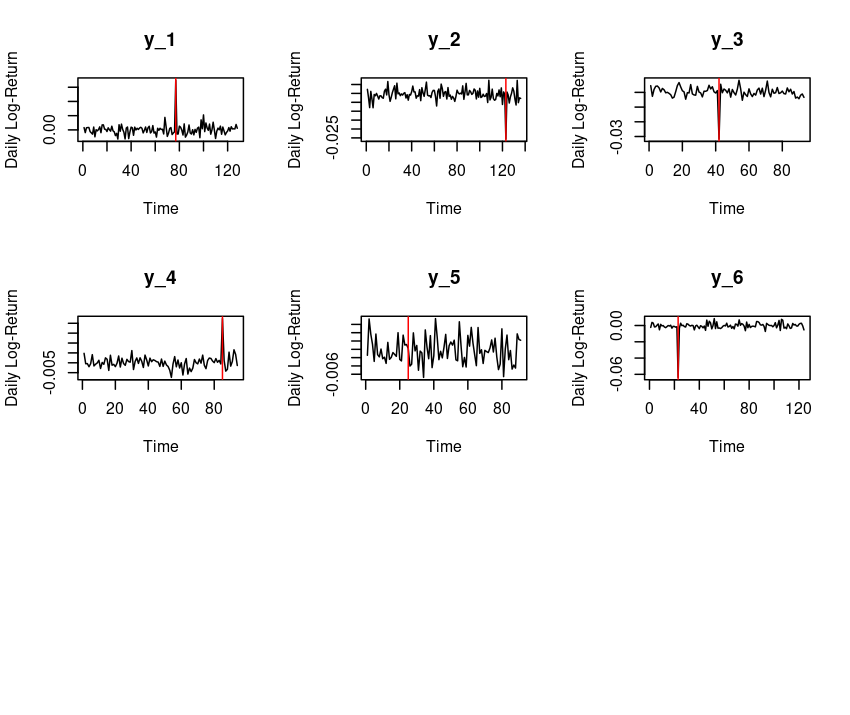
\includegraphics{level_shock.png}}
\caption{Above we see six simulations of GARCH processes that each manifest both a random shock to their observable level at some random time T*+1 and a random shock to their volatility (a latent quantity) at T*+1.}
\label{fig}
\end{figure}

\begin{figure}[htbp]
\centerline{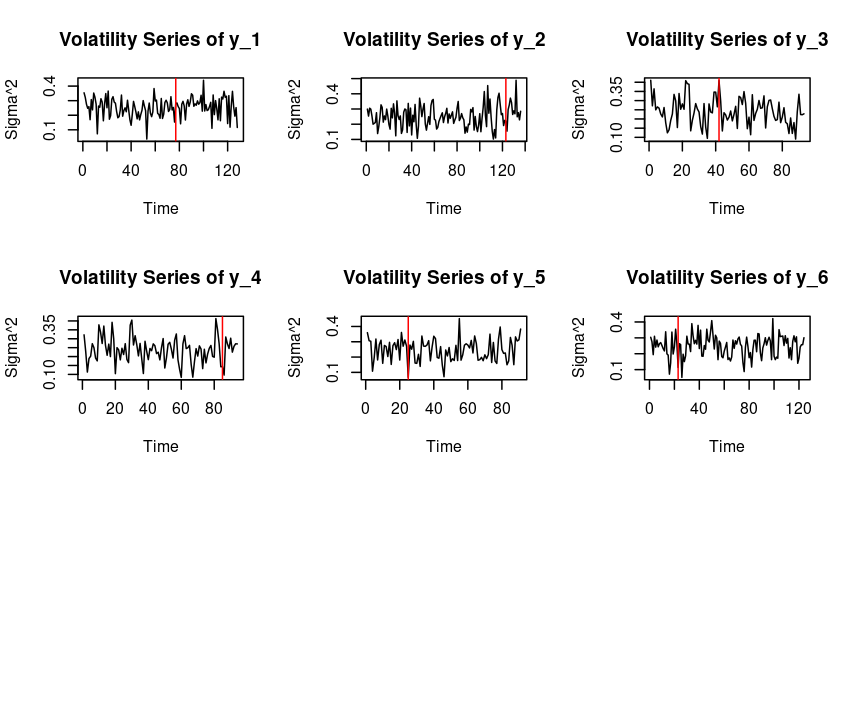
\includegraphics{vol_shock.png}}
\caption{Above we see the deterministic quantity $\sigma^{2}$ used to simulate the preceding GARCH processes.}
\label{fig}
\end{figure}

Notice that $\mc{M}_1$ assumes that $\omega^{*}_i$ are i.i.d. with $\E[ \omega^{*}_i]=\mu_{\omega^{*}}$ 
for $i = 1, \ldots, n+1$. We also consider a model where the shock effects are linear functions of covariates with an additional additive mean-zero error. For $i = 1, \ldots, n+1$, the random effects structure for this model (model $\mc{M}_2$) is:
\begin{align}
\mc{M}_2 \colon \begin{array}{l}
  y_{i,t} =\eta_i +\alpha_i D_{i,t} + \phi_i y_{i, t-1} + \theta_i'\mbf{x}_{i,t} + \varepsilon_{i,t}\\[.2cm]
  \; \alpha_i = \mu_{\alpha}+\delta_{i}'\mbf{x}_{i, T_i^*+1}+ \t{\varepsilon}_{i},
\end{array}\label{model2}
\end{align}
 where the added random effects are
\begin{align*}
\t{\varepsilon}_{i} &\simiid  \mc{F}_{\t{\varepsilon}} \text{ with }\mrm{E}_{\mc{F}_{\t{\varepsilon}}}(\t{\varepsilon}_{i})=0, \mrm{Var}_{\mc{F}_{\t{\varepsilon}}}(\t{\varepsilon}_{i})=\sigma^2_{\alpha} \where \sigma_{\alpha}>0\\
\eta_i &\indep  \alpha_i \indep \phi_i \indep \theta_i \indep \varepsilon_{i,t} \indep \t{\varepsilon}_{i}.
\end{align*} 
We further define 
$\tilde{\alpha}_i=\mu_{\alpha}+\delta_i'\mbf{x}_{i, T_i^*+1}$. 
We will investigate the post-shock aggregated estimators in $\mc{M}_2$ 
in settings where $\delta_i$ is either fixed or random. 
We let $\mc{M}_{21}$ denote model $\mc{M}_{2}$ with $\delta_i = \delta$ for $i= 1, \ldots, n+1$, 
where $\delta$ is a  fixed unknown parameter.
We let $\mc{M}_{22}$ denote model $\mc{M}_{2}$ with the following random effects 
structure for $\delta_i$:
\begin{align*}
\delta_i\simiid  \mc{F}_{\delta} \text{ with }\mrm{E}_{\mc{F}_{\delta}}(\delta_i)=\mu_{\delta}, \mrm{Var}_{\mc{F}_{\delta}}(\delta_i)=\Sigma_\delta 
   \quad \text{ with } \quad  \delta_i  \indep \t{\varepsilon}_{i}.
\end{align*}
We further define the parameter sets
\begin{align}
  \begin{array}{lll}
     \Theta &= &\{(\eta_i, \phi_i, \theta_i, \alpha_i, \mbf{x}_{i,t}, y_{i,t-1}, \delta_i)\colon t= 1, \ldots, T_i, i = 2, \ldots, n +1\},\\
    \Theta_1 &= &\{(\eta_i, \phi_i, \theta_i, \alpha_i, \mbf{x}_{i,t}, y_{i,t-1}, \delta_i)\colon t= 1, \ldots, T_i, i = 1\},\label{parameter}
  \end{array}
\end{align}
where $\Theta$ and $\Theta_1$ can adapt to $\mc{M}_1$ by dropping $\delta_i$. We assume this for notational simplicity.


We now describe the assumed autoregressive models with random effects for which post-shock aggregated estimators are provided. The model $\mc{M}$ is defined as
\begin{align}
\mc{M} \colon \begin{array}{l}
  y_{i,t} = \left(\eta_i + \sum_{j=1}^{q_1}\phi_{i,j}y_{i, t-j} + \sum_{j=0}^{q_2-1}\theta_{i,j+1}'\mbf{x}_{i,t-j}\right)(1 - D_{i,t}) + f(\mathcal{F}_{i,t},\alpha_i)D_{i,t} + \varepsilon_{i,t},\\[.2cm]
  \; f(\mc{F}_{i,t},\alpha_i) = \alpha_i +  \sum_{j=1}^{q_{1}}\t\phi_{i,j}y_{i, t-j} + \sum_{j=0}^{q_2-1}\t\theta_{i,j+1}'\mbf{x}_{i,t-j}, \\[.2cm]
  \; \alpha_i = \mu_{\alpha} + \delta_i'\mbf{x}_{i, T_i^*+1} + \varepsilon_{\alpha, i},
  %\sum_{j=1}^{q_3}\delta_{i,j}'\mbf{x}_{i, T_i^*-j+1}+ \t{\varepsilon}_{i}, 
\end{array}\label{model-gen}
\end{align}
where $D_{i,t} = I(t \geq T_i^* + 1)$, $I(\cdot)$ is the indicator function, $\x_{i,t} \in \R^{p}$ are fixed with $p \geq 1$. Let 
$\mathbf{\phi}_i = (\phi_{i,1},\ldots,\phi_{i,q_1})'$, 
$\mathbf{\theta}_i = (\theta_{i,1},\ldots,\theta_{i,q_2})'$, 
$\tilde{\mathbf{\phi}}_i = (\t\phi_{i,1},\ldots,\t\phi_{i,q_{1}})'$, 
$\tilde{\mathbf{\theta}}_i = (\t\theta_{i,1},\ldots,\t\theta_{i, q_{2}})'$, 
$\mathbf{\delta}_i = (\delta_{i,1},\ldots,\delta_{i,p})'$, 
and suppose that the regression coefficients in \eqref{model-gen} have the following hierarchical random effects structure: 
\begin{equation} \label{random-effects}
\begin{split}
  \eta_i &\simiid \mc{F}_{\eta} \text{ with }  \; \mrm{E}_{\mc{F}_{\eta}}(\eta_i) = \mu_\eta, \mrm{Var}_{\mc{F}_{\eta}}(\eta_i)  = \sigma^2_{\eta}, \\
  \mathbf{\phi}_{i,j} &\simiid \mc{F}_{\mathbf{\phi}_j} \text{ where } |\phi_{i,j}| < 1, \\
  \mathbf{\theta}_{i,j} &\simiid \mc{F}_{\mathbf{\theta}_j} \text{ with }  \; \mrm{E}_{\mc{F}_{\mathbf{\theta}_j}}(\theta_{i,j}) = \mu_{\mathbf{\theta}_j}, \mrm{Var}_{\mc{F}_{\mathbf{\theta}_j}}(\mathbf{\theta}_{i,j})  = \Sigma^2_{\mathbf{\theta}_j}, \\
  \mathbf{\delta}_i &\simiid  \mc{F}_{\mathbf{\delta}} \text{ with } \mrm{E}_{\mc{F}_{\mathbf{\delta}}}(\mathbf{\delta}_i)=\mu_{\mathbf{\delta}}, \mrm{Var}_{\mc{F}_{\mathbf{\delta}}}(\mathbf{\delta}_i)=\Sigma_{\mathbf{\delta}}, \\
\varepsilon_{i,t} & \simiid  \mc{F}_{\varepsilon_i} \text{ with }  \; \mrm{E}_{\mc{F}_{\varepsilon_i}}(\varepsilon_{i,t}) = 0, \mrm{Var}_{\mc{F}_{\varepsilon_i}}(\varepsilon_{i,t})  = \sigma^2_i,  \\
\varepsilon_{\alpha, i} &\simiid  \mc{F}_{\varepsilon_\alpha} \text{ with }\mrm{E}_{\mc{F}_{\varepsilon_\alpha}}(\varepsilon_{\alpha, i})=0, \mrm{Var}_{\mc{F}_{\varepsilon_{\alpha}}}(\varepsilon_{\alpha, i})=\sigma^2_{\alpha}, \\
  \tilde{\mathbf{\phi}}_{i,j} &\overset{ind}{\sim} \mathcal{F}_{\tilde{\mathbf{\phi}_j}}(\x_{i,T_i^*+1}) \; \text{where} \; |\tilde{\mathbf{\phi}}_{i,j}| < 1,  \\
  \tilde{\mathbf{\theta}}_{i,j} &\overset{ind}{\sim} \mathcal{F}_{\tilde{\mathbf{\theta}_j}}(\x_{i,T_i^*+1}),  \\  
 % \t q_{i,k} &\overset{ind}{\sim} \mathcal{F}_k(\x_{i,T_i^*}), \; k = 1,2, \\
&\eta_i \indep \mathbf{\phi}_{i,j} \indep \mathbf{\theta}_{i,j} \indep 
\tilde{\mathbf{\phi}}_{i,j} \indep \lambda_{i,j} \indep \mathbf{\delta}_i \indep \varepsilon_{i,t} \indep \tilde\varepsilon_{i}, 
\end{split}
\end{equation}
where the distributions $\mathcal{F}_{\tilde{\mathbf{\phi}}_j}(\x_{i,T_i^*+1})$ and $\mathcal{F}_{\tilde{\mathbf{\theta}}_{i'}}(\x_{i,T_i^*+1})$ satisfy $\mathcal{F}_{\tilde{\mathbf{\phi}}_j}(\x_{i,T_i^*+1}) \overset{d}{=} \mathcal{F}_{\tilde{\mathbf{\phi}}_{j}}(\x_{i',T_i^*+1})$ and $\mathcal{F}_{\tilde{\mathbf{\theta}}_j}(\x_{i,T_i^*+1}) \overset{d}{=} \mathcal{F}_{\tilde{\mathbf{\theta}}_{j}}(\x_{i',T_i^*+1})$ when $\x_{i,T_i^*+1} = \x_{i',T_i^*+1}$. Note that for model \eqref{model-gen} to be of use for post-shock forecasting, the variation in $\mathcal{F}_{\tilde{\mathbf{\phi}}}$ and $\mathcal{F}_{\tilde{\mathbf{\theta}}}$ must be small relative to the signal strength.


We see that model \eqref{model-gen} with its accompanying random effects structure \eqref{random-effects} is flexible enough to capture changing structural dynamics as well as a mean-shift, and is a generalization of the model in \cite{lin2021minimizing}. Note that the flexibility of allowing for changing structural dynamics is useful for fitting purposes, but it does not necessarily reflect the state of the world in the post-shock setting. It is of course possible that there is no shock or a simple mean-shift. 

The post-shock dynamic changes depend heavily on the value of $\mbf{x}_{i,T_i^*+1}$, the covariates recorded right before the first post-shock response is observed. Under this setup any two series $i,j$ with small $\|\mbf{x}_{i,T_i^*+1} - \mbf{x}_{j,T_i^*+1}\|_2$ are expected to experience similar structural changes. This makes distance based weighting an attractive avenue.



%We further define the parameter sets
%\begin{align}
%\begin{array}{l}
% \;\, \Theta = \{(\eta_i, \mathbf{\phi}_i, \mathbf{\theta}_i, \mathbf{\delta}_i, \alpha_i, \mbf{x}_{i,t}, y_{i,t-1})\colon    t= 1, \ldots, T_i, i = 2, \ldots, n +1\} \\
%   \Theta_1 = \{(\eta_i, \mathbf{\phi}_i, \mathbf{\theta}_i, \mathbf{\delta}_i, \alpha_i, \mbf{x}_{i,t}, y_{i,t-1})\colon  t= 1, \ldots, T_i, i = 1\}
%\end{array}\label{parameter} 
%\end{align}







\subsection{Forecasting and testing for shock persistence}
\label{forecast}


In this section, we motivates the relation between shock persistence testing and forecasting comparison. In time series literature, under a squared error loss $L(\cdot)$, the forecast using the conditional mean is the best point forecast that minimizes the expected loss if the model is specified correctly. That being said, even if the time series does experience a shock but the shock is not persistent, the expected loss of the conditional mean forecast should converge to the minimum expected loss that any forecast can achieve as sample size increases. On the other hand, if the shock is persistent, the conditional mean forecast that incorporates the shock information and makes good use of it should enjoy a smaller expected loss than any conditional mean forecast without such information does. In other words, the problem of testing for shock persistence boils down into comparing the conditional mean forecast that is adjusted by shock information and the one that is unadjusted. To deal with this problem, we applied the forecast comparison procedure of  \cite{quaedvlieg2021multi} to conduct shock persistence testing.

In this paper, we extend the framework of post-shock forecast \citep{lin2021minimizing}, which aggregates outside information by constructing a donor pool, to post-shock persistence testing. The donor pool consists of time series called  ``donors'' that are similar to the time series of interest. As we do not observe the future data, information from donors can aid our decision making and forecasts. Note that what  similarity exactly means here can be vague but the donors and the time series of interest should come from a common population in principle; see more details of how to select donors in \cite{lin2021minimizing}. In this paper, we also proposed several theoretical results with some detailed conditions on the donor pool, which may alleviate the difficulty of dealing with similarity when choosing donors.


In this paper, we propose a new way of aggregating information from donor pool to conduct post-shock persistence testing, which is quite different from \cite{lin2021minimizing}. The general structure of this aggregation technique is illustrated as below. Suppose we are given a nonempty donor pool with size $n$ that consists of donors $\mc{T}_2, \ldots, \mc{T}_{n+1}$, whose data, including shock information, are observed. With shock information, we are able to compute unadjusted forecast that does not incorporate shock information and adjusted forecast that does.  The forecast comparison using methodology of \cite{quaedvlieg2021multi} for each donor yields a $p$-value, $p_{i+1}$ for $i$th donor in the donor pool. Given $\{p_i \colon i = 2, \ldots, n+1\}$, we propose a methodology for judging whether the shock of the time series of interest is persistent or not. Next, we illustrate the details of our methodology as below.



For each donor $\mc{T}_i$, $i = 2, \ldots, n+1$, to compare adjusted and unadjusted forecasts,  a model needs to be specified. The model should describe how the shock impacts the time series at and after a certain time point $t= T_i^* + 1$. For clarity, we refers the unadjusted forecast to the conditional mean forecast based on the part of the model that ignores shock effect; and the adjusted forecast refers to the conditional mean forecast based on the full model. Note that the model needs not to be the same for every donor in the donor pool. However, certain conditions need to be imposed as discussed previously. 

 Given a model for each donor pool, we compute the unadjusted conditional mean forecast and adjusted conditional mean forecast in the framework of \cite{quaedvlieg2021multi}. As introduced in the beginning of Section \ref{section2}, for a given horizon $h$, to forecast $y_{i, t}$, we compute the two forecasts based on the information set $\mathcal{F}_{i, t-h}$ of each donor pool (i.e., the data before $t-h$) for $i = 2, \ldots, n+1$. Note that in practice, a training sample size $K_i$ should be specified for $i = 2, \ldots, n+1$ such that we use the information set $\mathcal{F}_{i, t-h-K_i + 1:t-h}$. 
 
 Even if the data contain shock information for each donor, it is impossible to compute the adjusted conditional mean forecast based on $\mathcal{F}_{i, t-h}$ when $t -h \leq T_i^*$, i.e., we only have training data that do no have any shock information. Note that this is not a big problem when $t-h \geq T_i^* +1$ because  $\mathcal{F}_{i, t-h}$ starts to incorporate shock information. In the literature, \cite{lin2021minimizing} utilizes donor pool information to provide an consistent estimator of the shock effect such that the adjusted  conditional mean forecast is the unadjusted one plus the shock effect estimate. However, the consistent estimation comes with the cost of assuming certain models (in terms of first and second moments) for the shock effect across the donor pool and the method only works for additive shock effect model.  To our best knowledge, there  is no other available methods that can accommodate the case when the shock model is nonlinear. However, even if the model is misspecified, using additive shock effect model to approximate the scalar shock effect that occurs at $t=T_i^*+1$ may still help as opposed to doing nothing. 
 
 With the presence of autoregressive parameters in some models, unbiased estimation with OLS  is not feasible but the bias is $O(T^{-1})$, where $T$ is the time series length \citep{shaman1988bias}. In this paper, we use the OLS estimates to approximate the adjusted conditional mean forecast and unadjusted one. The bias decades away as $T\to \infty$.

\vspace*{0.5cm}

\noindent\textbf{Note}: Our forecast needs to be written with respect to our general model. Specifics can be given when we conduct our numerical examples.
\vspace*{0.5cm}

In our post-shock setting we consider the following candidate forecasts: 
\begin{align*}
  &\text{Forecast 1}: \\
  &\text{Forecast 2}: 
\end{align*}
We want to determine which forecast is appropriate over a horizon while the methods in \cite{lin2021minimizing} were only appropriate in the nowcasting setting in which prediction was only focused on the response immediately following the shock.





\newpage

\noindent\textbf{Note}: We need to explain what the voting method is, possibly in algorithmic format. Also note that the p-values that we obtain are computed using a bootstrap procedure. Perhaps an additional proposition that states the performance of these bootstrap p-values would further guarantee reliability. 

\begin{prop}

\label{votprop}Suppose $p_2, \ldots, p_{n+1}$ is  a sequence of pairwise independent $p$-values  with $\P(p_i \leq \alpha)=\kappa$ for $i = 1, \ldots, n+1$, where $\alpha$ is the significance level, $\kappa$ is a real-valued constant in $[0,1]$, and  $p_1$ is the p-value of the time series of interest. If $\P(p_1 \leq \alpha) \neq 0.5$,
\begin{align*}
  \E \bigg\{\left|I\left\{\frac{1}{n}\sum_{i=2}^{n+1}I(p_i \leq  \alpha) \geq 0.5\right\}
  - I( p_1 \leq  \alpha) \right|\bigg\}
  \to  \begin{cases}
    1- \P(p_1 \leq \alpha) & \text{ if } \P(p_1 \leq \alpha) > 0.5 \\
    \P(p_1 \leq \alpha) & \text{ if } \P(p_1 \leq \alpha) < 0.5 
  \end{cases}
\end{align*}
\end{prop}

\begin{proof}
Notice that as $\P(p_i \leq \alpha)=\kappa$ for $i = 1, \ldots, n+1$ and $I(p_i \leq  \alpha) $ is a Bernoulli random variable, $I(p_i \leq  \alpha)$ is identically distributed for  $i = 1, \ldots, n+1$. Since $p_i$ is pairwise independent and $p_i$ are identically distributed for $i = 2, \ldots, n+1$, by Weak Law of Large Numbers, 
\begin{align*}
  \frac{1}{n}\sum_{i=2}^{n+1}I(p_i \leq  \alpha)  
   \stackrel{p}{\rightarrow}  \P(p_i \leq \alpha) = \P(p_1 \leq \alpha),
\end{align*}
Define
\begin{align*}
  f \colon [0,1] \mapsto \{0,1\} 
  \text{ with }
  f(x) = I(x \geq 0.5).
\end{align*}
Let $C(f)$ denote the continuity set of $f$. Suppose that $\P(p_1 \leq  \alpha) \neq 0.5$. In this case, notice that 
\begin{align*}
  \P(\P(p_1 \leq  \alpha) \in C(f)) =1.
\end{align*}
By Slutsky's Theorem, we have
\begin{align*}
  I\left\{\frac{1}{n}\sum_{i=2}^{n+1}I(p_i \leq  \alpha) \geq 0.5\right\}
  \stackrel{p}{\rightarrow} 
  I\{ \P(p_1 \leq  \alpha) \geq 0.5\}.
\end{align*}
It follows that
\begin{align*}
   I\left\{\frac{1}{n}\sum_{i=2}^{n+1}I(p_i \leq  \alpha) \geq 0.5\right\}- I( p_1 \leq  \alpha) 
  \stackrel{p}{\rightarrow} 
  I\{ \P(p_1 \leq  \alpha) \geq 0.5\} - I( p_1 \leq  \alpha) 
\end{align*}
Since the function $g(x)= |x|$ is continuous in $x$,  by continuous mapping theorem, 
\begin{align*}
  \bigg|  I\left\{\frac{1}{n}\sum_{i=2}^{n+1}I(p_i \leq  \alpha) \geq 0.5\right\}
  - I( p_1 \leq  \alpha) \bigg| \stackrel{p}{\rightarrow}   |I\{ \P(p_1 \leq  \alpha) \geq 0.5\}
  - I( p_1 \leq  \alpha) |
\end{align*}
Moreover, note that
\begin{align*}
\E \left\{ |I\{ \P(p_1 \leq  \alpha) \geq 0.5\}
  - I( p_1 \leq  \alpha) |\right\}
  & = \begin{cases}
    1- \P(p_1 \leq \alpha) & \text{ if } \P(p_1 \leq \alpha) > 0.5 \\
    \P(p_1 \leq \alpha) & \text{ if } \P(p_1 \leq \alpha) < 0.5 
  \end{cases} \\
  & \leq  0.5.
\end{align*}
Due to the fact that
\begin{align*}
 \left|I\left\{\frac{1}{n}\sum_{i=2}^{n+1}I(p_i \leq  \alpha) \geq 0.5\right\}
  - I( p_1 \leq  \alpha) \right| \leq 1
\end{align*}
is bounded by 1, by Dominated Convergence Theorem for the version of convergence in measure,
\begin{align*}
 \left|I\left\{\frac{1}{n}\sum_{i=2}^{n+1}I(p_i \leq  \alpha) \geq 0.5\right\}
  - I( p_1 \leq  \alpha) \right|
  \stackrel{\mathcal{L}_1}{\rightarrow}  |I\{ \P(p_1 \leq  \alpha) \geq 0.5\}
  - I( p_1 \leq  \alpha) |.
\end{align*}
That would imply that 
\begin{align*}
  \E \bigg\{\left|I\left\{\frac{1}{n}\sum_{i=2}^{n+1}I(p_i \leq  \alpha) \geq 0.5\right\}
  - I( p_1 \leq  \alpha) \right|\bigg\}
  \to  \begin{cases}
    1- \P(p_1 \leq \alpha) & \text{ if } \P(p_1 \leq \alpha) > 0.5 \\
    \P(p_1 \leq \alpha) & \text{ if } \P(p_1 \leq \alpha) < 0.5 
  \end{cases}
\end{align*}
That is, the expected misclassification rate of voting converges to 
\begin{align*}
  \begin{cases}
    1- \P(p_1 \leq \alpha) & \text{ if } \P(p_1 \leq \alpha) > 0.5 \\
    \P(p_1 \leq \alpha) & \text{ if } \P(p_1 \leq \alpha) < 0.5 
  \end{cases}
\end{align*}
\end{proof}

\begin{lem}
  \label{gwlln}  For each $n\in \naturals$, let $c_{n1}, \ldots, c_{nn}$ be real numbers bounded by some $K > 0$, and let $X_{n1}, \ldots, X_{nn}$ be pairwise independent random variables defined on a probability space $(\Omega_n, \mc{F}_n, \P_n)$, and let $\E_n$ and $\var_n$ denote the corresponding expectation and variance. If $(b_n)$ is a sequence of positive numbers such that $b_n \uparrow \infty$ such that
    \begin{align*}
      \sum_{i=1}^n \P_n (|X_{ni}| > b_n) \to 0
      \quad \text{ and } 
      \quad \frac{1}{(b_n)^2} \sum_{i=1}^n \E_n[X_{ni}^2; |X_{ni}|\leq b_n] \to 0,
    \end{align*}
    then
    \begin{align*}
      \frac{1}{b_n} \sum_{i=1}^n c_{ni} (X_{ni} - \E_n[X_{ni}; X_{ni} \leq b_n]) \cp 0.
    \end{align*}
\end{lem}

\begin{proof}
  For each $n\in \naturals$ set
    \begin{align*}
      S_n = \sum_{i=1}^n c_{ni} X_{ni}, \quad T_n = \sum_{i=1}^n c_{ni} Y_{ni},
      \quad Y_{ni} = X_{ni} I(|X_{ni}|\leq b_n), \quad i = 1, \ldots, n.
    \end{align*}
   The goal is to show that  $(S_n- \E_n[T_n])/b_n \cp 0$. For this, it suffices to show that (1) $(T_n - S_n)/b_n \cp 0$ and (2) $(T_n - \E_n[T_n])/b_n \cp 0$ because
    \begin{align*}
      (T_n - \E_n[T_n])/b_n -(T_n - S_n)/b_n = (S_n- \E_n[T_n])/b_n .
    \end{align*}
     We first prove (1). Notice that for every $\varepsilon > 0$ and $n\in \naturals$,
    \begin{align*}
      \{|S_n- T_n| > \varepsilon\}\subseteq \bigcup_{i=1}^n \{X_{ni}\neq Y_{ni}\}
      = \bigcup_{i=1}^n \{|X_{ni}|>b_n\},
    \end{align*}
    and, as a result, by Boole's inequality we have
    \begin{align*}
      \P_n (|S_n - T_n|>\varepsilon) \leq \sum_{i=1}^n \P_n(|X_{ni}|>b_n) \to 0,
    \end{align*}
    which proves (1). Next, we prove (2). Since $\mc{L}^2$ implies convergence in probability, it suffices to show that $(T_n-\E[T_n])/b_n \clt 0$, i.e., $\var[T_n]/(b_n)^2 \to 0$. Since $X_{n1}, \ldots, X_{nn}$ are pairwise independent, so are $Y_{n1}, \ldots, Y_{nn}$, and consequently
    \begin{align*}
      \Var_n[T_n]=\sum_{i=1}^n \Var_n[Y_{ni}] \leq \sum_{i=1}^n \E_n[(c_{ni}X_{ni})^2; |X_{ni}|\leq b_n] \leq K^2\sum_{i=1}^n \E_n[(X_{ni})^2; |X_{ni}|\leq b_n].
    \end{align*}
    As a result,
    \begin{align*}
    0\leq   \frac{\Var_n[T_n]}{b_n^2}\leq K^2 \cdot  \frac{1}{b_n^2}\sum_{i=1}^n \E_n[(X_{ni})^2; |X_{ni}|\leq b_n] \to 0,
    \end{align*}
    which proves the result by sandwich theorem.
\end{proof}


\begin{corollary}
\label{coro1}Let $(w_2, \ldots, w_{n+1})$ be weights such that $w_i \in [0,1]$ and $\sum_{i=2}^{n+1} w_i=1$. Define
\begin{align*}
  \mc{I}_n = \{i = \in 2,\ldots, n+1\colon 0< w_i < 1\}.
\end{align*}
Suppose that  $\mc{I}_n$  is non-empty, $|\mc{I}_n| \to \infty$ as $n \to \infty$, and $w_i b_n\leq K$ for $i\in \mc{I}_n$ and some $K>0$, where $b_n \geq 1$ and $b_n \to \infty$ as $n\to \infty$. Assume for $i \in \mc{I}_n$,  $p_i$ are pairwise independent $p$-values  with 
\begin{align*}
  \sum_{i\in \mc{I}_n}\P(p_i \leq \alpha) = \sum_{i\in \mc{I}_n} w_i \kappa_i \to \kappa_{1},
\end{align*}
where $\kappa_i =  \P(p_i \leq \alpha)\in [0,1]$ for $i \in \mc{I}_n$, $\alpha$ is the significance level, $\kappa_1 = \P(p_1 \leq \alpha)$, and  $p_1$ is the p-value of the time series of interest. If $\P(p_1 \leq \alpha) \neq 0.5$,
\begin{align*}
  \E \bigg\{\left|I\left\{ \sum_{i\in \mc{I}_n} w_i I(p_i \leq  \alpha) \geq 0.5\right\}
  - I( p_1 \leq  \alpha) \right|\bigg\}
  \to  \begin{cases}
    1- \P(p_1 \leq \alpha) & \text{ if } \P(p_1 \leq \alpha) > 0.5 \\
    \P(p_1 \leq \alpha) & \text{ if } \P(p_1 \leq \alpha) < 0.5 
  \end{cases}
\end{align*}
\end{corollary}

\begin{proof}
  The proof is rather similar to Proposition \ref{votprop}. It suffices to show that
  \begin{align*}
   \sum_{i\in \mc{I}_n} w_i I(p_i \leq  \alpha) \cp \kappa_1 =  \P(p_1 \leq \alpha).
  \end{align*}
  and the remaining proof is the same as that of Proposition \ref{votprop} in terms of applying Dominated Convergence Theorem in the version of  convergence in probability. As $p_i$ are pairwise independent for $i\in \mc{I}_n$, $I(p_i\leq \alpha)$ are pairwise independent for $i \in \mc{I}_n$. The idea is to prove the required condition of Lemma \ref{gwlln} holds. As  $\mc{I}_n$  is non-empty, $|\mc{I}_n| \to \infty$, $b_n > 1$, and  $b_n \to \infty$ as $n \to \infty$, 
  \begin{align*}
    & \sum_{i\in \mc{I}_n} \P\big( I(p_i \leq  \alpha) > b_n\big) \to 0\\
   & \frac{1}{b_n^2} \sum_{i\in \mc{I}_n} \E\big[ I(p_i \leq  \alpha) \,|\, I(p_i \leq  \alpha) \leq b_n\big]
     =  \frac{1}{b_n^2} \sum_{i\in \mc{I}_n} \P\big(p_i \leq\alpha \big)
     = \frac{1}{b_n^2} \sum_{i\in \mc{I}_n} w_i \kappa_i  \to 0
  \end{align*}
  because $ \sum_{i\in \mc{I}_n} w_i \kappa_i = O(1)$ by the assumption $\sum_{i\in \mc{I}_n} w_i \kappa_i \to \kappa_{1}$. Let $c_{ni} = w_i b_n$ for $i \in \mc{I}_n$. Since $w_i b_n\leq K$ for some $K > 0$ and $b_n$, we have 
  \begin{align*}
    & \frac{1}{b_n} \sum_{i\in \mc{I}_n}  c_{ni} \big(  I(p_i \leq  \alpha) - \P( I(p_i \leq  \alpha) \, |\,  I(p_i \leq  \alpha)  \leq b_n )  \big) \\
  = \quad     &\frac{1}{b_n} \sum_{i\in \mc{I}_n}  c_{ni} \big(  I(p_i \leq  \alpha) - \P( I(p_i \leq  \alpha) \big)  \cp 0
  \end{align*}
  which follows from Lemma \ref{gwlln}. The above is equivalent to
  \begin{align*}
   \sum_{i\in \mc{I}_n}  w_i I(p_i \leq  \alpha) - \sum_{i\in \mc{I}_n} w_i  \kappa_i  \cp 0
  \end{align*}
  As $\sum_{i\in \mc{I}_n} w_i  \kappa_i\to \kappa_1$ as $n \to \infty$, by Slutsky's Theorem,
  \begin{align*}
     \sum_{i\in \mc{I}_n}  w_i I(p_i \leq  \alpha)  \cp \kappa_1,
  \end{align*}
  which finishes the proof.
\end{proof}






\newpage

\vspace*{0.5cm} We now demonstrate an idealized theoretical setting for which our post-shock testing methodology involving a distance based weighted average of p-values works well. The idea is that inferences based on distance based weighted nearly recovers the time series under study when there exists a time series in the donor pool, indexed by $i'$, such that $\x_{1,t} \approx \x_{i',t}$ and the signal strength in our modeling setup \eqref{model-gen} and \eqref{random-effects} is large relative to variation. We first present some intermediary technical results and definitions. Let $\lambda_{\text{max},\theta_k}$, $\lambda_{\text{max},\theta_\delta}$, $\lambda_{\text{max},\gamma}$ respectively be the largest eigenvalues of $\Sigma_{\theta_k}$, $\Sigma_{\delta}$, and $\Sigma_{\gamma}$ for $k = 1,\ldots,q_2$. Define  
\begin{align*}
  \mu_{\min} &= \min\left(\mu_\eta,\mu_{\phi_j},\mu_{\tilde\phi_j},\min(\mu_\delta),\min(\mu_{\theta_k}),\min(\mu_{\tilde\theta_k}); j = 1,\ldots,q_1, k = 1,\ldots,q_2\right), \\
  \mu_{\max} &= \max\left(\mu_\eta,\mu_{\phi_j},\mu_{\tilde\phi_j},\max(\mu_\delta),\max(\mu_{\theta_k}),\max(\mu_{\tilde\theta_k}); j = 1,\ldots,q_1, k = 1,\ldots,q_2\right), \\
  \lambda_{\max} &= \max\left(\lambda_{\text{max},\theta_k}, \lambda_{\text{max},\theta_\delta}, \lambda_{\text{max},\gamma}; k = 1,\ldots,q_2\right), \\
  \sigma^2_{\max} &= \max\left(\sigma^2_{\eta},\sigma^2_{\phi_j},\sigma^2_i,\sigma^2_{\alpha},\sigma^2_{\tilde{\phi}_j}; i = 1,\ldots,n+1, j = 1,\ldots,q_1\right).  
\end{align*}



\begin{prop} \label{prop:signaltonoise}
  Let $\bf{y}_{i,t}$, $i = 1,\ldots,n_i$, $t = 1,\ldots, T$ be a collection of independent time series. Let each time series $\bf{y}_{i,t}$ be generated by model \eqref{model-gen} with accompanying random effects structure \eqref{random-effects}, where $y_{i,t}$ is a scalar response $\x_{i,t} \in \R^p$ is a fixed vector of covariates. Suppose that there is a common shock time $p + 2 < T^* < T - (p+2)$ where $q_1 = q_2 = 1$, $\|\x_{i,t}\| = 1$, each entry of $\x_{i,t}$ is non-negative, $\mu_{\min} > 0$, and $y_{i,0} = 0$. Then for every $1 \leq t \leq T$ we have that 
  \begin{equation} \label{signal-to-noise}
    \E(y_{i,t}) \geq C\Var(y_{i,t}),  
  \end{equation}
  provided that 
  \begin{equation} \label{condition-1}
  \begin{split}
    \mu_\alpha + 3\mu_{\min} &\geq C\left(3\sigma^2_{\max} + 2\lambda_{\max}\right), \\
    2\mu_{\min} &\geq C\left(2\sigma^2_{\max} + \lambda_{\max}\right).  
  \end{split}
  \end{equation}
\end{prop}


\textbf{Remarks}:
\begin{enumerate}
  \item The conditions \eqref{condition-1} govern the signal strength necessary in the expected behavior of the underlying random effects structure relative to variability necessary for the overall signal to noise ratio for the overall time series to be lower bounded by some positive value $C$.
  \item The conditions of Proposition~\ref{prop:signaltonoise} state that there is an increasing trend in $y_{i,t}$ for all $i$. This can be relaxed, but a fully general argument is cumbersome.
\end{enumerate}



\begin{proof}
For $t > T^* + 1$ we have 
\begin{align*}
  \E(y_{i,t}) &= \E\left[\E(y_{i,t}|y_{i,t-1})\right] \\ 
    &= \E\left[\E(\eta_i + \alpha_i + \tilde\phi_i y_{i,t-1} 
      + \tilde\theta_i'\x_{i,t}|y_{i,t-1})\right] \\
    &= \E(\eta_i + \mu_\alpha + \delta_i'\x_{i,T^*+1} + \tilde\phi_i y_{i,t-1} + \tilde\theta_i'\x_{i,t}) \\
    &= \mu_\eta + \mu_\alpha + \mu_\delta'\x_{i,T^*+1} + \mu_{\tilde\theta}'\x_{i,t} + \mu_{\tilde\phi}\E(y_{i,t-1}) \\
    &\geq (\mu_\alpha + 3\mu_{\min}) + \mu_{\min}\E(y_{i,t-1}) \\
    &\geq \sum_{j=1}^{t - (T^* + 1)} \mu_{\min}^j(\mu_{\alpha} + 3\mu_{\min}) + \mu_{\min}^{t-T^*}\E(y_{i,T^*}) \\
    &= \sum_{j=0}^{t - (T^* + 1)} \mu_{\min}^j(\mu_{\alpha} + 3\mu_{\min}) + \mu_{\min}^{t-T^*}\left(\E\left[\E(y_{i,T^*}|y_{i,T^*-1})\right]\right) \\   
    &= \sum_{j=0}^{t - (T^* + 1)} \mu_{\min}^j(\mu_{\alpha} + 3\mu_{\min}) + \mu_{\min}^{t-T^*}\left(\E(\eta_i + \theta_i'\x_{i,T^*} + \phi_i y_{i,T^*-1}) \right) \\
    &\geq \sum_{j=0}^{t - (T^* + 1)} \mu_{\min}^j(\mu_{\alpha} + 3\mu_{\min}) + \mu_{\min}^{t-T^*}\left(2\mu_{\min} + \mu_{\min} \E(y_{i,T^*-1}) \right) \\
    &\geq \sum_{j=0}^{t - (T^* + 1)} \mu_{\min}^j(\mu_{\alpha} + 3\mu_{\min}) + \mu_{\min}^{t-T^*}\left(\sum_{j=0}^{T^*-1}\mu_{\min}^j(2\mu_{\min}) \right), 
\end{align*}
and 
\begin{align*}
  \Var(y_{i,t}) &= \E\left[\Var(y_{i,t}|y_{i,t-1})\right] + \Var\left[\E(y_{i,t}|y_{i,t-1})\right] \\
  &= \E\left[\Var(\eta_i + \mu_\alpha + \delta_i'\x_{i,T^*+1} + \tilde\theta_i'\x_{i,t} + \tilde\phi_i y_{i,t-1} + \varepsilon_{i,t} + \varepsilon_{\alpha,i}|y_{i,t-1})\right] \\
  &+ \Var\left[\E(\eta_i + \mu_\alpha + \delta_i'\x_{i,T^*+1} + \tilde\theta_i'\x_{i,t} + \tilde\phi_i y_{i,t-1} + \varepsilon_{i,t} + \varepsilon_{\alpha,i}|y_{i,t-1})\right] \\
  &\leq 3\sigma^2_{\max} + 2\lambda_{\max} + \Var\left[\E(\tilde\phi_i y_{i,t-1}|y_{i,t-1})\right] \\
  &= 3\sigma^2_{\max} + 2\lambda_{\max} + \mu_{\tilde\phi}^2\Var(y_{i,t-1}) \\
  &\leq \sum_{j=0}^{t - (T^*+1)} (\mu_{\tilde\phi}^2)^j\left(3\sigma^2_{\max} + 2\lambda_{\max}\right) + (\mu_{\tilde\phi}^2)^{t - T^*}\Var(y_{i,T^*}) \\
  &= \sum_{j=0}^{t - (T^*+1)} (\mu_{\tilde\phi}^2)^j\left(3\sigma^2_{\max} + 2\lambda_{\max}\right) + (\mu_{\tilde\phi}^2)^{t - T^*}\left(\E\left[\Var(y_{i,T^*}|y_{i,T^*-1})\right] + \Var\left[\E(y_{i,T^*}|y_{i,T^*-1})\right]\right) \\
  &= \sum_{j=0}^{t - (T^*+1)} (\mu_{\tilde\phi}^2)^j\left(3\sigma^2_{\max} + 2\lambda_{\max}\right) + (\mu_{\tilde\phi}^2)^{t - T^*}\left(\E\left[\Var(\eta_i + \theta_i'\x_{i,T^*} + \phi_iy_{i,T^*-1} + \varepsilon_{i,T^*}|y_{i,T^*-1})\right] \right. \\ 
  &\qquad+  \left.\Var\left[\E(\eta_i + \theta_i'\x_{i,T^*} + \phi_iy_{i,T^*-1} + \varepsilon_{i,T^*}|y_{i,T^*-1})\right]\right)  \\
  &\leq \sum_{j=0}^{t - (T^*+1)} (\mu_{\tilde\phi}^2)^j\left(3\sigma^2_{\max} + 2\lambda_{\max}\right) + (\mu_{\tilde\phi}^2)^{t - T^*}\left(2\sigma^2_{\max} + \lambda_{\max} + \mu_{\phi}^2\Var(y_{i,T^*-1}) \right) \\ 
  &\leq \sum_{j=0}^{t - (T^*+1)} (\mu_{\tilde\phi}^2)^j\left(3\sigma^2_{\max} + 2\lambda_{\max}\right) + (\mu_{\tilde\phi}^2)^{t - T^*}\left(\sum_{j=0}^{T^*-1}\left(\mu_{\phi}^2\right)^{j}(2\sigma^2_{\max} + \lambda_{\max})\right).  
\end{align*}
Combining the above with the condition \eqref{condition-1} yields 
\begin{align*}
  \frac{\E(y_{i,t})}{\Var(y_{i,t})} &\geq \frac{\sum_{j=0}^{t - (T^* + 1)} \mu_{\min}^j(\mu_{\alpha} + 3\mu_{\min}) + \mu_{\min}^{t-T^*}\left(\sum_{j=0}^{T^*-1}\mu_{\min}^j(2\mu_{\min}) \right)}{\sum_{j=0}^{t - (T^*+1)} (\mu_{\tilde\phi}^2)^j\left(3\sigma^2_{\max} + 2\lambda_{\max}\right) + (\mu_{\tilde\phi}^2)^{t - T^*}\left(\sum_{j=0}^{T^*-1}\left(\mu_{\phi}^2\right)^{j}(2\sigma^2_{\max} + \lambda_{\max})\right)} \\
  &\geq \frac{C\sum_{j=0}^{t - (T^*+1)} (\mu_{\tilde\phi}^2)^j\left(3\sigma^2_{\max} + 2\lambda_{\max}\right) + C(\mu_{\tilde\phi}^2)^{t - T^*}\left(\sum_{j=0}^{T^*-1}\left(\mu_{\phi}^2\right)^{j}(2\sigma^2_{\max} + \lambda_{\max})\right)}{\sum_{j=0}^{t - (T^*+1)} (\mu_{\tilde\phi}^2)^j\left(3\sigma^2_{\max} + 2\lambda_{\max}\right) + (\mu_{\tilde\phi}^2)^{t - T^*}\left(\sum_{j=0}^{T^*-1}\left(\mu_{\phi}^2\right)^{j}(2\sigma^2_{\max} + \lambda_{\max})\right)} \\
  &= C,
\end{align*}
for all $i$ and $t$. A similar argument holds when $t \leq T^* + 1$.
\end{proof}


\begin{lem}[Technical Lemma 1] \label{lem:absdiff}
Let $a_j, b_j \in \R$, $j = 1,2$ be such that $0 < a_1,a_2 < 1$, $b_1,b_2 > 0$. Let $c_1 = \max(a_1,a_2)$, $c_2 = \min(a_1,a_2)$, $d_1 = \max(b_1,b_2)$, $d_2 = \min(b_1,b_2)$. Then, 
$$
  |a_1b_1 - a_2b_2| \leq |a_1 - a_2|d_1 + |b_1 - b_2|c_2.
$$
\end{lem}

\begin{proof}
Observe that 
$$
  |a_1b_1 - a_2b_2| \leq c_1d_1 - c_2d_2 = (c_1 - c_2)d_1 + (d_1 - d_2)c_2. 
$$
The conclusion follows by noting that $c_1 - c_2 = |a_1 - a_2|$ and $d_1 - d_2 = |b_1 - b_2|$.
\end{proof}


\begin{prop} \label{prop:donor}
  Let $\bf{y}_{i,t}$, $i = 1,\ldots,n_i$, $t = 1,\ldots, T$ be a collection of independent time series. Let each time series $\bf{y}_{i,t}$ be generated by model \eqref{model-gen} with accompanying random effects structure \eqref{random-effects}, where $y_{i,t}$ is a scalar response $\x_{i,t} \in \R^p$ is a fixed vector of covariates. Suppose that there is a common shock time $p + 2 < T^* < T - (p+2)$ where $q_1 = q_2 = 1$, $\|\x_{i,t}\| = 1$, each entry of $\x_{i,t}$ is non-negative, $\mu_{\min} > 0$, and $y_{i,0} = 0$. Let $i' \geq 2$ be an index. Then, for any $\epsilon > 0$ we can choose an $\gamma > 0$ such that 
  $$
    \left\vert\E(y_{i,t} - y_{i',t})\right\vert \leq \epsilon, \qquad |\Var(y_{1,t}) - \Var(y_{i',t})| < \varepsilon,
  $$
  provided that 
  \begin{align*}
  |\mu_\delta'\x_{1,T^*+1} - \mu_\delta'\x_{i',T^*+1}| &< \gamma, \\
%  |\mu_{\tilde\theta_1}'\x_{1,T^*+1} - \mu_{\tilde\theta_{i'}}'\x_{i',T^*+1}| &< \gamma, \\
  \left\vert\mu_{\tilde\theta_{1}}'\x_{1,t} - \mu_{\tilde\theta_{i'}}'\x_{i',t}\right\vert &< \gamma, \qquad \text{for all} \; t, \\
  |\mu_{\tilde\phi_1}^j - \mu_{\tilde\phi_{i'}}^j| &< \gamma, \qquad \text{for all} \; j, \\
  |\x_{1,T^*+1}'\Sigma_\delta\x_{1,T^*+1} - \x_{i',T^*+1}'\Sigma_\delta\x_{i',T^*+1}| &< \gamma, \\
  |\x_{1,t}'\Sigma_{\tilde\theta_{1}}\x_{1,t} - \x_{i',t}'\Sigma_{\tilde\theta_{i'}}\x_{i',t}| &< \gamma, \qquad \text{for all} \; t.
  \end{align*}
\end{prop}

\begin{proof}
A similar recursion to that seen in the proof of Proposition~\ref{prop:signaltonoise} yields
\begin{align*}
  &|\E(y_{1,t} - y_{i',t})| =  \left\vert \sum_{j=0}^{t - (T^*+1)}\left[\left(\mu_{\tilde\phi_{1}}^j(\mu_\delta'\x_{1,T^*+1}) - \mu_{\tilde\phi_{i'}}^j(\mu_\delta'\x_{i',T^*+1})\right) + \mu_{\tilde\phi_{1}}^j(\mu_{\tilde\theta_{1}}'\x_{1,t-j}) - \mu_{\tilde\phi_{i'}}^j(\mu_{\tilde\theta_{i'}}'\x_{i',t-j})\right]\right. \\
    &\qquad\qquad\left. + \sum_{j=0}^{T^* - 1}\left[\mu_\eta(\mu_{\tilde\phi_{1}}^{t - T^*} - \mu_{\tilde\phi_{i'}}^{t - T^*})\mu_{\phi}^j + \left(\mu_{\tilde\phi_{1}}^{t - T^*}(\mu_{\theta}'\x_{1,t-j}) - \mu_{\tilde\phi_{i'}}^{t - T^*}(\mu_{\theta}'\x_{i',t-j})\right)\mu_{\phi}^j\right]\right\vert \\
  &\qquad\leq |\mu_\delta'\x_{1,T^*+1} - \mu_\delta'\x_{i',T^*+1}| 
    + \sum_{j=1}^{t - (T^*+1)}\left\vert\mu_{\tilde\phi_{1}}^j(\mu_\delta'\x_{1,T^*+1}) - \mu_{\tilde\phi_{i'}}^j(\mu_\delta'\x_{i',T^*+1})\right\vert \\ 
  &\qquad\qquad+ |\mu_{\tilde\theta_{1}}'\x_{1,t} - \mu_{\tilde\theta_{i'}}'\x_{i',t}| + \sum_{j=1}^{t - (T^*+1)}\left\vert \mu_{\tilde\phi_{1}}^j(\mu_{\tilde\theta_{1}}'\x_{1,t-j}) - \mu_{\tilde\phi_{i'}}^j(\mu_{\tilde\theta_{i'}}'\x_{i',t-j})\right\vert \\
  &\qquad\qquad + \mu_\eta\sum_{j=0}^{T^*-1}\left\vert \mu_{\tilde\phi_{1}}^{t - T^*} - \mu_{\tilde\phi_{i'}}^{t - T^*}\right\vert\mu_{\phi}^j + \sum_{j=0}^{T^*-1}\left\vert \mu_{\tilde\phi_{1}}^{t - T^*}(\mu_{\theta}'\x_{1,T^*-j}) - \mu_{\tilde\phi_{i'}}^{t - T^*}(\mu_{\theta}'\x_{i',T^*-j}) \right\vert\mu_{\phi}^j \\
  &\qquad\leq |\mu_\delta'\x_{1,T^*+1} - \mu_\delta'\x_{i',T^*+1}| + |\mu_{\tilde\theta_{1}}'\x_{1,t} - \mu_{\tilde\theta_{i'}}'\x_{i',t}| \\
  &\qquad\qquad + \sum_{j=1}^{t - (T^*+1)}\left[\vert\mu_{\tilde\phi_{1}}^j - \mu_{\tilde\phi_{i'}}^j\vert\max(\mu_\delta'\x_{1,T^*+1},\mu_\delta'\x_{i',T^*+1}) + \left\vert\mu_\delta'\x_{1,T^*+1} -\mu_\delta'\x_{i',T^*+1}\right\vert\mu_{\tilde\phi_{1}}^j\right] \\
  &\qquad\qquad + \sum_{j=1}^{t - (T^*+1)}\left[\vert\mu_{\tilde\phi_{1}}^j - \mu_{\tilde\phi_{i'}}^j\vert\max(\mu_\delta'\x_{1,t-j},\mu_\delta'\x_{i',t-j}) + \left\vert\mu_{\tilde\theta_{1}}'\x_{1,t-j} - \mu_{\tilde\theta_{i'}}'\x_{i',t-j}\right\vert\mu_{\tilde\phi_{1}}^j\right] \\
  &\qquad\qquad + \mu_\eta\sum_{j=0}^{T^*-1}\left\vert \mu_{\tilde\phi_{1}}^{t - T^*} - \mu_{\tilde\phi_{i'}}^{t - T^*}\right\vert\mu_{\phi}^j + \sum_{j=0}^{T^*-1}\left\vert \mu_{\tilde\phi_{1}}^{t - T^*}(\mu_{\theta}'\x_{1,T^*-j}) - \mu_{\tilde\phi_{i'}}^{t - T^*}(\mu_{\theta}'\x_{i',T^*-j}) \right\vert\mu_{\phi}^j,  
\end{align*}
where the second inequality follows from applications of Lemma~\ref{lem:absdiff}. Continuing from the second inequality, the conditions of this proposition imply that
\begin{align*}
  &|\E(y_{1,t} - y_{i',t})| \\
  &\qquad\leq 2\gamma + \sum_{j=1}^{\infty}\left[\vert\mu_{\tilde\phi_{1}}^j - \mu_{\tilde\phi_{i'}}^j\vert\max(\mu_\delta'\x_{1,T^*+1},\mu_\delta'\x_{i',T^*+1}) + \gamma\mu_{\tilde\phi_{1}}^j\right] \\
  &\qquad\qquad + \sum_{j=1}^{\infty}\left[\vert\mu_{\tilde\phi_{1}}^j - \mu_{\tilde\phi_{i'}}^j\vert\max(\mu_\delta'\x_{1,t-j},\mu_\delta'\x_{i',t-j}) + \gamma\mu_{\tilde\phi_{1}}^j\right] \\
  &\qquad\qquad + \mu_\eta\sum_{j=0}^{\infty}\left\vert \mu_{\tilde\phi_{1}}^{t - T^*} - \mu_{\tilde\phi_{i'}}^{t - T^*}\right\vert\mu_{\phi}^j + \sum_{j=0}^{\infty}\left\vert \mu_{\tilde\phi_{1}}^{t - T^*}(\mu_{\theta}'\x_{1,T^*-j}) - \mu_{\tilde\phi_{i'}}^{t - T^*}(\mu_{\theta}'\x_{i',T^*-j}) \right\vert\mu_{\phi}^j  \\
  &\qquad\leq 2\gamma + 2\gamma\frac{\max(\mu_\delta)}{(1 - \mu_{\tilde\phi_{1}})(1 - \mu_{\tilde\phi_{i'}})} \\
  &\qquad\qquad + \mu_\eta\sum_{j=0}^{\infty}\left\vert \mu_{\tilde\phi_{1}}^{t - T^*} - \mu_{\tilde\phi_{i'}}^{t - T^*}\right\vert\mu_{\phi}^j + \sum_{j=0}^{\infty}\left\vert \mu_{\tilde\phi_{1}}^{t - T^*}(\mu_{\theta}'\x_{1,T^*-j}) - \mu_{\tilde\phi_{i'}}^{t - T^*}(\mu_{\theta}'\x_{i',T^*-j}) \right\vert\mu_{\phi}^j \\
  &\qquad\leq 2\gamma + 2\gamma\frac{\max(\mu_\delta)}{(1 - \mu_{\tilde\phi_{1}})(1 - \mu_{\tilde\phi_{i'}})} + \gamma\frac{\mu_{\eta}}{1 - \mu_{\phi}} + \sum_{j=0}^{\infty}\left\vert \mu_{\tilde\phi_{1}}^{t - T^*}(\mu_{\theta}'\x_{1,T^*-j}) - \mu_{\tilde\phi_{i'}}^{t - T^*}(\mu_{\theta}'\x_{i',T^*-j}) \right\vert\mu_{\phi}^j \\
  &\qquad\leq 2\gamma + 2\gamma\frac{\max(\mu_\delta)}{(1 - \mu_{\tilde\phi_{1}})(1 - \mu_{\tilde\phi_{i'}})} + \gamma\frac{\mu_{\eta}}{1 - \mu_{\phi}} + \gamma\frac{\max(\mu_\theta) + 1}{1 - \mu_\phi}, 
\end{align*}  
where the last inequality follows from Lemma~\ref{lem:absdiff}. We can choose $\gamma$ small enough so that $|\E(y_{1,t} - y_{i',t})| < \varepsilon$. A similar recursion for the variance yields 
\begin{align*}
 &\left\vert \Var(y_{1,t}) - \Var(y_{i',t})\right\vert 
   = \left\vert \x_{1,T^*+1}'\Sigma_\delta\x_{1,T^*+1} - \x_{i',T^*+1}'\Sigma_\delta\x_{i',T^*+1} + \x_{1,t}'\Sigma_{\tilde\theta_i}\x_{1,t} -   \x_{i',t}'\Sigma_{\tilde\theta_{i'}}\x_{i',t} \right. \\
   &\qquad\left. + \mu_{\tilde\phi_1}^2\Var(y_{1,t-1}) - \mu_{\tilde\phi_{i'}}^2\Var(y_{i',t-1}) \right\vert \\
   &\leq \left\vert \x_{1,T^*+1}'\Sigma_\delta\x_{1,T^*+1} - \x_{i',T^*+1}'\Sigma_\delta\x_{i',T^*+1} + \x_{1,t}'\Sigma_{\tilde\theta_i}\x_{1,t} -   \x_{i',t}'\Sigma_{\tilde\theta_{i'}}\x_{i',t}\right\vert \\
   &\qquad + \left\vert\mu_{\tilde\phi_1}^2\Var(y_{1,t-1}) - \mu_{\tilde\phi_{i'}}^2\Var(y_{i',t-1})\right\vert \\
   &= \left\vert \x_{1,T^*+1}'\Sigma_\delta\x_{1,T^*+1} - \x_{i',T^*+1}'\Sigma_\delta\x_{i',T^*+1} + \x_{1,t}'\Sigma_{\tilde\theta_1}\x_{1,t} -   \x_{i',t}'\Sigma_{\tilde\theta_{i'}}\x_{i',t}\right\vert \\
   &\qquad + \left\vert \mu_{\tilde\phi_1}^2\left(\sigma^2_\eta + \sigma^2_{\alpha}+ \sigma^2 + \x_{1,T^*+1}'\Sigma_\delta\x_{1,T^*+1} + \x_{1,t-1}'\Sigma_{\tilde\theta_1}\x_{1,t-1} + \mu_{\tilde\phi_1}^2\Var(y_{1,t-2})\right) \right.\\
   &\qquad\qquad\left.- \mu_{\tilde\phi_{i'}}^2\left(\sigma^2_\eta + \sigma^2_{\alpha}+ \sigma^2 + \x_{i',T^*+1}'\Sigma_\delta\x_{i',T^*+1} + \x_{i',t-1}'\Sigma_{\tilde\theta_{i'}}\x_{i',t-1} + \mu_{\tilde\phi_{i'}}^2\Var(y_{i',t-2})\right) \right\vert \\
   &\leq \left\vert \x_{1,T^*+1}'\Sigma_\delta\x_{1,T^*+1} - \x_{i',T^*+1}'\Sigma_\delta\x_{i',T^*+1}\right\vert + \left\vert\x_{1,t}'\Sigma_{\tilde\theta_1}\x_{1,t} -   \x_{i',t}'\Sigma_{\tilde\theta_{i'}}\x_{i',t}\right\vert \\ 
   &\qquad+ \left\vert \mu_{\tilde\phi_1}^2\left(\sigma^2_\eta + \sigma^2_{\alpha}+ \sigma^2 + \x_{1,T^*+1}'\Sigma_\delta\x_{1,T^*+1} + \x_{1,t-1}'\Sigma_{\tilde\theta_1}\x_{1,t-1}\right) \right.\\
   &\qquad\qquad\left.- \mu_{\tilde\phi_{i'}}^2\left(\sigma^2_\eta + \sigma^2_{\alpha}+ \sigma^2 + \x_{i',T^*+1}'\Sigma_\delta\x_{i',T^*+1} + \x_{i',t-1}'\Sigma_{\tilde\theta_{i'}}\x_{i',t-1}\right) \right\vert \\
   &\qquad + \left\vert \mu_{\tilde\phi_1}^4\Var(y_{1,t-2}) - \mu_{\tilde\phi_{i'}}^4\Var(y_{i',t-2}) \right\vert \\
   &\leq \sum_{j=0}^{t - (T^* + 1)}\left[ \left\vert \mu_{\tilde\phi_1}^{2j}\x_{1,T^*+1}'\Sigma_\delta\x_{1,T^*+1} - \mu_{\tilde\phi_{i'}}^{2j}\x_{i',T^*+1}'\Sigma_\delta\x_{i',T^*+1}\right\vert \right. \\
   &\qquad\left. + \left\vert \mu_{\tilde\phi_1}^{2j}\x_{1,t-j}'\Sigma_{\tilde\theta_1}\x_{1,t-j} - \mu_{\tilde\phi_{i'}}^{2j}\x_{i',t-j}'\Sigma_{\tilde\theta_{i'}}\x_{i',t-j} \right\vert + \left\vert\mu_{\tilde\phi_1}^{2j} - \mu_{\tilde\phi_{i'}}^{2j}\right\vert(\sigma^2_\eta + \sigma^2_{\alpha}+ \sigma^2)\right] \\
   &\qquad + \left\vert \mu_{\tilde\phi_1}^{2(t - T^*)}\Var(y_{1,t - T^*}) - \mu_{\tilde\phi_{i'}}^{2(t - T^*)}\Var(y_{i',t - T^*}) \right\vert \\
   &\leq \sum_{j=0}^{t - (T^* + 1)}\left[ \left\vert \mu_{\tilde\phi_1}^{2j} - \mu_{\tilde\phi_{i'}}^{2j}\right\vert \lambda_{\text{max}} +  \left\vert\x_{1,T^*+1}'\Sigma_\delta\x_{1,T^*+1} - \x_{i',T^*+1}'\Sigma_\delta\x_{i',T^*+1}\right\vert\mu_{\tilde\phi_1}^{2j} \right. \\
   &\qquad\left. + \left\vert \mu_{\tilde\phi_1}^{2j} - \mu_{\tilde\phi_{i'}}^{2j}\right\vert \lambda_{\text{max}} +  \left\vert\x_{1,t-j}'\Sigma_{\tilde\theta_1}\x_{1,t-j} - \x_{i',t-j}'\Sigma_{\tilde\theta_{i'}}\x_{i',t-j}\right\vert\mu_{\tilde\phi_1}^{2j} + \left\vert\mu_{\tilde\phi_1}^{2j} - \mu_{\tilde\phi_{i'}}^{2j}\right\vert(\sigma^2_\eta + \sigma^2_{\alpha}+ \sigma^2)\right] \\
   &\qquad + \left\vert \mu_{\tilde\phi_1}^{2(t - T^*)}\sum_{j=0}^{T^*-1}\left(\sigma^2_\eta + \sigma^2 + \x_{1,T^*-j}'\Sigma_\theta\x_{1,T^*-j}\right)\mu_{\phi}^{2j} \right. \\ 
   &\qquad\qquad\left. - \mu_{\tilde\phi_{i'}}^{2(t - T^*)}\sum_{j=0}^{T^*-1}\left(\sigma^2_\eta + \sigma^2 + \x_{i',T^*-j}'\Sigma_\theta\x_{i',T^*-j}\right)\mu_{\phi}^{2j} \right\vert \\
   &\leq 2\gamma\frac{\lambda_{\max}}{(1 - \mu_{\tilde\phi_1}^{2})(1 - \mu_{\tilde\phi_{i'}}^{2})} + 2\gamma\frac{1}{1 - \mu_{\tilde\phi_1}^2} + \gamma\frac{\sigma^2_\eta + \sigma^2_{\alpha}+ \sigma^2}{(1 - \mu_{\tilde\phi_1}^{2})(1 - \mu_{\tilde\phi_{i'}}^{2})} \\
   &\qquad+ (\sigma^2_\eta + \sigma^2)\left\vert \mu_{\tilde\phi_1}^{2(t - T^*)} - \mu_{\tilde\phi_{i'}}^{2(t - T^*)} \right\vert\sum_{j=0}^{T^*-1}\mu_{\phi}^{2j} \\
   &\qquad+ \sum_{j=0}^{2(t - T^*)}\left\vert \mu_{\tilde\phi_1}^{2(t - T^*)}\x_{1,T^*-j}'\Sigma_\theta\x_{1,T^*-j} - \mu_{\tilde\phi_{i'}}^{2(t - T^*)}\x_{i',T^*-j}'\Sigma_\theta\x_{i',T^*-j} \right\vert \mu_{\phi}^{2j} \\
   &\leq 2\gamma\frac{\lambda_{\max}}{(1 - \mu_{\tilde\phi_1}^{2})(1 - \mu_{\tilde\phi_{i'}}^{2})} + 2\gamma\frac{1}{1 - \mu_{\tilde\phi_1}^2} + \gamma\frac{\sigma^2_\eta + \sigma^2_{\alpha}+ \sigma^2}{(1 - \mu_{\tilde\phi_1}^{2})(1 - \mu_{\tilde\phi_{i'}}^{2})} \\ 
   &\qquad + \gamma\frac{\sigma^2_\eta + \sigma^2}{1 - \mu_\phi^2} + \gamma\frac{\lambda_{\max}}{1 - \mu_\phi^2} + \gamma\frac{1}{1 - \mu_\phi^2}
   \end{align*}
We can choose $\gamma$ small enough so that $|\Var(y_{1,t}) - \Var(y_{i',t})| < \varepsilon$.
\end{proof}

\begin{lem}[Technical Lemma 2] \label{lem:diffsig2noise}
Let $a_j, b_j \in \R$, $j = 1,2$. Suppose that $b_j > b > 0$ for $j = 1,2$. Then for any $\varepsilon > 0$ we have 
$$
  \left\vert\frac{a_1}{b_1} - \frac{a_2}{b_2}\right\vert \leq \varepsilon,
$$
provided that $|a_1-a_2|$,$|b_1-b_2| < \delta$ for some chosen $\delta > 0$.
\end{lem}

\begin{proof}
\begin{align*}
  \left\vert\frac{a_1}{b_1} - \frac{a_2}{b_2}\right\vert 
    &= \left\vert\frac{a_1b_2 - a_2b_1}{b_1b_2}\right\vert 
    = \left\vert\frac{(a_1 - a_2 + a_2)(b_2 - b_1 + b_1) - a_2b_1}{b_1b_2}\right\vert \\
    &= \left\vert \frac{a_1(b_2 - b_1) + a_2b_1 + (a_1 - a_2)b_1 - a_2b_1}{b_1b_2} \right\vert \leq \frac{2\delta}{b^2} \\
    &\leq \frac{|a_1|\delta + |b_1|\delta}{b^2} \leq \varepsilon, 
\end{align*}
where $\delta \leq \varepsilon b^2/(|a_1| + |b_1|)$.
\end{proof}

\begin{cor} \label{cor:differences}
  Let $\bf{y}_{i,t}$, $i = 1,\ldots,n_i$, $t = 1,\ldots, T$ be a collection of independent time series. Let each time series $\bf{y}_{i,t}$ be generated by model \eqref{model-gen} with accompanying random effects structure \eqref{random-effects}, where $y_{i,t}$ is a scalar response $\x_{i,t} \in \R^p$ is a fixed vector of covariates. Suppose that there is a common shock time $p + 2 < T^* < T - (p+2)$ where $q_1 = q_2 = 1$, $\|\x_{i,t}\| = 1$, each entry of $\x_{i,t}$ is non-negative, $\mu_{\min} > 0$, and $y_{i,0} = 0$. Let $i' \geq 2$ be an index. Assume that $\Var(y_{1,t})$, $\Var(y_{i',t}) \geq b$ for all $t$.  Assume the conditions of Proposition~\ref{prop:donor}. Then we can choose an $\varepsilon > 0$ such that 
  $$
    \left\vert \frac{\E(y_{1,t})}{\Var(y_{1,t})} - \frac{\E(y_{i',t})}{\Var(y_{i',t})} \right\vert \leq \varepsilon,
  $$
  for all $1 \leq t \leq T$.
\end{cor}

\begin{proof}
  From Proposition~\ref{prop:donor} we can pick an arbitrary number $\delta > 0$ such that $\left\vert\E(y_{i,t} - y_{i',t})\right\vert \leq \delta$ and $|\Var(y_{1,t}) - \Var(y_{i',t})| < \delta$ for all $t = 1,\ldots,T$. The conclusion follows from Lemma~\ref{lem:diffsig2noise}.
\end{proof}

This is some justification for the idea that one may be able to make inferences about the time series of interest using a time series from the donor pool. 

\vspace*{0.5cm}

\noindent \textbf{Doodles}:
\begin{align*}
  &\Prob\left(\left\vert |y_{1,t} - \E(y_{1,t})| - |y_{i',t} - \E(y_{i',t})| \right\vert \leq \varepsilon_1\right) 
  \geq \Prob\left(|y_{1,t} - \E(y_{1,t})| \leq \varepsilon_1/2,  |y_{i',t} - \E(y_{i',t})| \leq \varepsilon_1/2\right) \\
  &\qquad = \Prob\left(|y_{1,t} - \E(y_{1,t})| \leq \varepsilon_1/2\right) \Prob\left(|y_{i',t} - \E(y_{i',t})| \leq \varepsilon_1/2\right) \\
  &\qquad \geq \left(1 - \frac{4\Var(y_{1,t})}{\varepsilon_1^2}\right)\left(1 - \frac{4\Var(y_{i',t})}{\varepsilon_1^2}\right) \\
  &\qquad \geq \left(1 - \frac{4\E(y_{1,t})}{\varepsilon_1^2C}\right)\left(1 - \frac{4\E(y_{i',t})}{\varepsilon_1^2C}\right),
  %&\qquad = 1 - \frac{4\E(y_{1,t})}{\varepsilon^2C} - \frac{4\E(y_{i',t})}{\varepsilon^2C} + \frac{16\E(y_{1,t})\E(y_{i',t})}{\varepsilon^4C^2},
\end{align*}
for all $t = 1,\ldots,T$ where the second inequality follows from Chebyshev's inequality and the last inequality follows from Proposition~\ref{prop:signaltonoise}.

\vspace*{0.5cm}
The above argument implies that a $C$ can be chosen so that 
\begin{align*}
  &|y_{1,t} - y_{i',t}| = |y_{1,t} - y_{i',t} \pm \E(y_{1,t}) \pm \E(y_{i',t})| \\
  &\qquad = |(y_{1,t} - \E(y_{1,t})) - (y_{i',t} - \E(y_{i',t})) + (\E(y_{1,t}) - \E(y_{i',t}))| \\
  &\qquad \leq |y_{1,t} - \E(y_{1,t})| + |y_{i',t} - \E(y_{i',t})| + |\E(y_{1,t}) - \E(y_{i',t})| \\
  &\qquad \leq \varepsilon_2,
\end{align*}
holds with high probability for all $t = 1,\ldots,T$ by Proposition~\ref{prop:donor}.

\vspace*{0.5cm}
Add condition that $\text{argmax}_t\|\x_{1,t} - \x_{i',t}\| < \delta$. Then the OLS estimates satisfy 
$$
  \|(\hat\eta_1,\hat\phi_1,\hat\theta_1',\hat\alpha_1)' - 
    (\hat\eta_{i'},\hat\phi_{i'},\hat\theta_{i'}',\hat\alpha_{i'})'\| < \varepsilon_3
$$
with high probability, and therefore $\left\vert|y_{1,t} - \hat y_{i,t}| - |y_{i',t} - \hat y_{i',t}|\right\vert < \varepsilon_4$ with high probability for all $t = 1,\ldots,T$.






\section{Simulation Setup}
\label{simulation}

Let $n$ denote the donor pool size, $p$ denote the number of covariates used, $H$ denote the number of horizon used, $T_i$ denote the length of time series to be evaluated for time series $i$, $K_i$ denote the training sample size used for each  forecasting  time series $i$, $T_i^*$ denote the time point just before the realization of the shock for time series $i$ for $i = 1, \ldots, n+1$.


In this setting $n$, $p$, and $H$ are pre-determined. $T_i, K_i \sim \mrm{Gamma}(15, 10)$.  The total sample size for $i$th time series is $T_i + K_i + H$. $T_i^*$ is randomly sampled from $\ceil{\frac{1}{4}T_i}+1$ to $\ceil{\frac{3}{4} T_i} + K_i+ H$. If $T_i, K_i < 90$, we force them to be 90. The adopted model for the data is as below:
\begin{align*}
  y_{i,t} &= \eta_i + \phi_i y_{i,t-1} + \mbf{x}_{i,t} \bs{\beta}_i + \alpha_i I(t > T_i^*) + \varepsilon_{i,t},\\
  \alpha_i &= \mu_{\alpha} + \mbf{x}_{i,T_i^*+1}\bs{\gamma}_i + \tilde{\varepsilon}_{i},
\end{align*}
where
\begin{align*}
  \phi_i & \sim \text{ indep. }  U(0,1) \\
  \eta_i & \sim \text{ indep. }  \mc{N}(0,1) \\
  \varepsilon_{i,t} & \sim \text{ indep. } \mc{N}(0, \sigma^2)\\
  \tilde{\varepsilon}_i & \sim \text{ indep. } \mc{N}(0, \sigma_{\alpha}^2)
  \\
  \bs{\gamma}_i & \sim \text{ indep. } \mc{N}(\mu_{\gamma}\bs{1}_p, \sigma_{\gamma}^2 \mbf{I}_p) \\
  \bs{\beta}_i & \sim \text{ indep. }  \mc{N}(\bs{0}_p, \mbf{I}_p).
\end{align*}
Moreover, the elements of $\mathbf{x}_{i,t}$ are independently distributed as $\mrm{Gamma}(1,\delta)$.

Note that $K_i$ is training sample size for time series $i$. Consider
\begin{align*}
  K_i & \sim \ceil{\mrm{Gamma}(a_{K}, b_K)}\\
   T_i & \sim \ceil{\mrm{Gamma}(a_{T}, b_T)} \\
  T_i^* &\equiv \max\{T_i+1, \ceil{0.5 \cdot(T_i+K_i+H)}\},
\end{align*}

$K_i+H+T_i^* > T_i+K_i+H$

 Then, we consider the following simulation setup
\begin{verbatim}
  ns <- c(5, 10, 20, 40)
  Tscale <- Kscale <- 1 / 2 # b_T, b_K 
  K.T.shape <- c(200, 400, 800, 1600) # for K_i and T_i
  mu.gamma.delta <- 2 # mean for parameter vector of shock
  sigma.delta.gamma <- 0.1 # sd for parameter vector of shock
  sigma.alpha <- 0.05 # sd for shock noise  
  sigma <- 0.1 # sd for response noise
  mu.alpha <- 50 # intercept for shock (relatively large)
  H <- 8 
  ell <- 4
  scale <- 2 # scale for covariates that follow Gamma distribution
\end{verbatim}

\begin{align*}
  y_{i,t} &= \eta_i + \phi_i y_{i,t-1} + \mbf{x}_{i,t} \bs{\beta}_i + \xi_i\cdot  I(t > T_i^*) + \varepsilon_{i,t},\\
  \xi_i &= \alpha_i \cdot e^{-(t-T_i^*-1)} \\
  \alpha_i &= \mu_{\alpha} + \mbf{x}_{i,T_i^*+1}\bs{\gamma}_i + \tilde{\varepsilon}_{i},
\end{align*}









\bibliographystyle{plainnat}
\bibliography{synthVolForecast}
%\bibliography{../synthetic-prediction-notes}

  
\end{document}


